%% LyX 2.3.4.2 created this file.  For more info, see http://www.lyx.org/.
%% Do not edit unless you really know what you are doing.
\documentclass[english,dvipsnames,aspectratio=169,handout]{beamer}
\usepackage{mathptmx}
\usepackage{eulervm}
\usepackage[T1]{fontenc}
\usepackage[latin9]{inputenc}
\usepackage{babel}
\usepackage{amstext}
\usepackage{amssymb}
\usepackage{graphicx}
\usepackage{ifthen}
\usepackage{xcolor}
\usepackage{xspace}
\usepackage{tikz}
\usetikzlibrary{tikzmark}
\usetikzlibrary{calc}
\usepackage{pgfplots}
%\pgfplotsset{compat=1.17}
\usepackage{booktabs}
\usepackage{xpatch}
\usepackage{multirow}
\usepackage{colortbl}
\usepackage{pgfpages}




\xpatchcmd{\itemize}
  {\def\makelabel}
  {\ifnum\@itemdepth=1\relax
     \setlength\itemsep{2ex}% separation for first level
   \else
     \ifnum\@itemdepth=2\relax
       \setlength\itemsep{1ex}% separation for second level
     \else
       \ifnum\@itemdepth=3\relax
         \setlength\itemsep{0.5ex}% separation for third level
   \fi\fi\fi\def\makelabel
  }
 {}
 {}

\ifx\hypersetup\undefined
  \AtBeginDocument{%
    \hypersetup{unicode=true,pdfusetitle,
 bookmarks=true,bookmarksnumbered=false,bookmarksopen=false,
 breaklinks=false,pdfborder={0 0 0},pdfborderstyle={},backref=false,colorlinks=true,
 allcolors=NYUPurple,urlcolor=LightPurple}
  }
\else
  \hypersetup{unicode=true,pdfusetitle,
 bookmarks=true,bookmarksnumbered=false,bookmarksopen=false,
 breaklinks=false,pdfborder={0 0 0},pdfborderstyle={},backref=false,colorlinks=true,
 allcolors=NYUPurple,urlcolor=LightPurple}
\fi

\makeatletter

%%%%%%%%%%%%%%%%%%%%%%%%%%%%%% LyX specific LaTeX commands.
%% Because html converters don't know tabularnewline
\providecommand{\tabularnewline}{\\}

%%%%%%%%%%%%%%%%%%%%%%%%%%%%%% Textclass specific LaTeX commands.
% this default might be overridden by plain title style
\newcommand\makebeamertitle{\frame{\maketitle}}%
% (ERT) argument for the TOC
\AtBeginDocument{%
  \let\origtableofcontents=\tableofcontents
  \def\tableofcontents{\@ifnextchar[{\origtableofcontents}{\gobbletableofcontents}}
  \def\gobbletableofcontents#1{\origtableofcontents}
}

%%%%%%%%%%%%%%%%%%%%%%%%%%%%%% User specified LaTeX commands.
\usetheme{CambridgeUS} 
\beamertemplatenavigationsymbolsempty


% Set Color ==============================
\definecolor{NYUPurple}{RGB}{87,6,140}
\definecolor{LightPurple}{RGB}{165,11,255}


\setbeamercolor{title}{fg=NYUPurple}
\setbeamercolor{frametitle}{fg=NYUPurple}

\setbeamercolor{background canvas}{fg=NYUPurple, bg=white}
\setbeamercolor{background}{fg=black, bg=NYUPurple}

\setbeamercolor{palette primary}{fg=black, bg=gray!30!white}
\setbeamercolor{palette secondary}{fg=black, bg=gray!20!white}
\setbeamercolor{palette tertiary}{fg=gray!20!white, bg=NYUPurple}

\setbeamertemplate{headline}{}
\setbeamerfont{itemize/enumerate body}{}
\setbeamerfont{itemize/enumerate subbody}{size=\normalsize}

\setbeamercolor{parttitle}{fg=NYUPurple}
\setbeamercolor{sectiontitle}{fg=NYUPurple}
\setbeamercolor{sectionname}{fg=NYUPurple}
\setbeamercolor{section page}{fg=NYUPurple}
%\setbeamercolor{description item}{fg=NYUPurple}
%\setbeamercolor{block title}{fg=NYUPurple}

\setbeamertemplate{blocks}[rounded][shadow=false]
\setbeamercolor{block body}{bg=normal text.bg!90!NYUPurple}
\setbeamercolor{block title}{bg=NYUPurple!30, fg=NYUPurple}



\AtBeginSection[]{
  \begin{frame}
  \vfill
  \centering
\setbeamercolor{section title}{fg=NYUPurple}
 \begin{beamercolorbox}[sep=8pt,center,shadow=true,rounded=true]{title}
    \usebeamerfont{title}\usebeamercolor[fg]{title}\insertsectionhead\par%
  \end{beamercolorbox}
  \vfill
  \end{frame}
}

\makeatother

\setlength{\parskip}{\medskipamount} 

\input ../macros

\begin{document}
\input ../rosenberg-macros

%\setbeameroption{show notes on second screen}

\title[DS-GA 1003]{Gaussian Mixture Model}
\author{He He \\
Slides based on Lecture
\href{https://github.com/davidrosenberg/mlcourse/blob/gh-pages/Lectures/13b.mixture-models.pdf}{13b} from David Rosenberg's course materials (\url{https://github.com/davidrosenberg/mlcourse})
}
\date{April 27, 2021}
\institute{CDS, NYU}

\makebeamertitle
\mode<article>{Just in article version}

\begin{frame}{Probabilistic Model for Clustering}
\onslide<1->{
\begin{columns}
\begin{column}{0.55\textwidth}
\begin{itemize}
\item Problem setup: 
\begin{itemize}
\item There are $k$ clusters (or \textbf{mixture components}).
\item We have a probability distribution for each cluster.
\end{itemize}
}

\onslide<2->{
\item Generative story of a \textbf{mixture distribution}:
\begin{enumerate}
\item Choose a random cluster $z\in\left\{ 1,2,\ldots,k\right\} $. 
\item Choose a point from the distribution for cluster $z$. 
\end{enumerate}
\end{itemize}
}
\end{column}

\onslide<3->{
\begin{column}{0.4\textwidth}
\begin{simpleblock}
{Example:}
\begin{enumerate}
\item Choose $z\in\left\{ 1,2,3\right\} $ with $p(1)=p(2)=p(3)=\frac{1}{3}$. 
\item Choose $x\mid z\sim\cn\left(X\mid\mu_{z},\Sigma_{z}\right)$.
\end{enumerate}
\end{simpleblock}

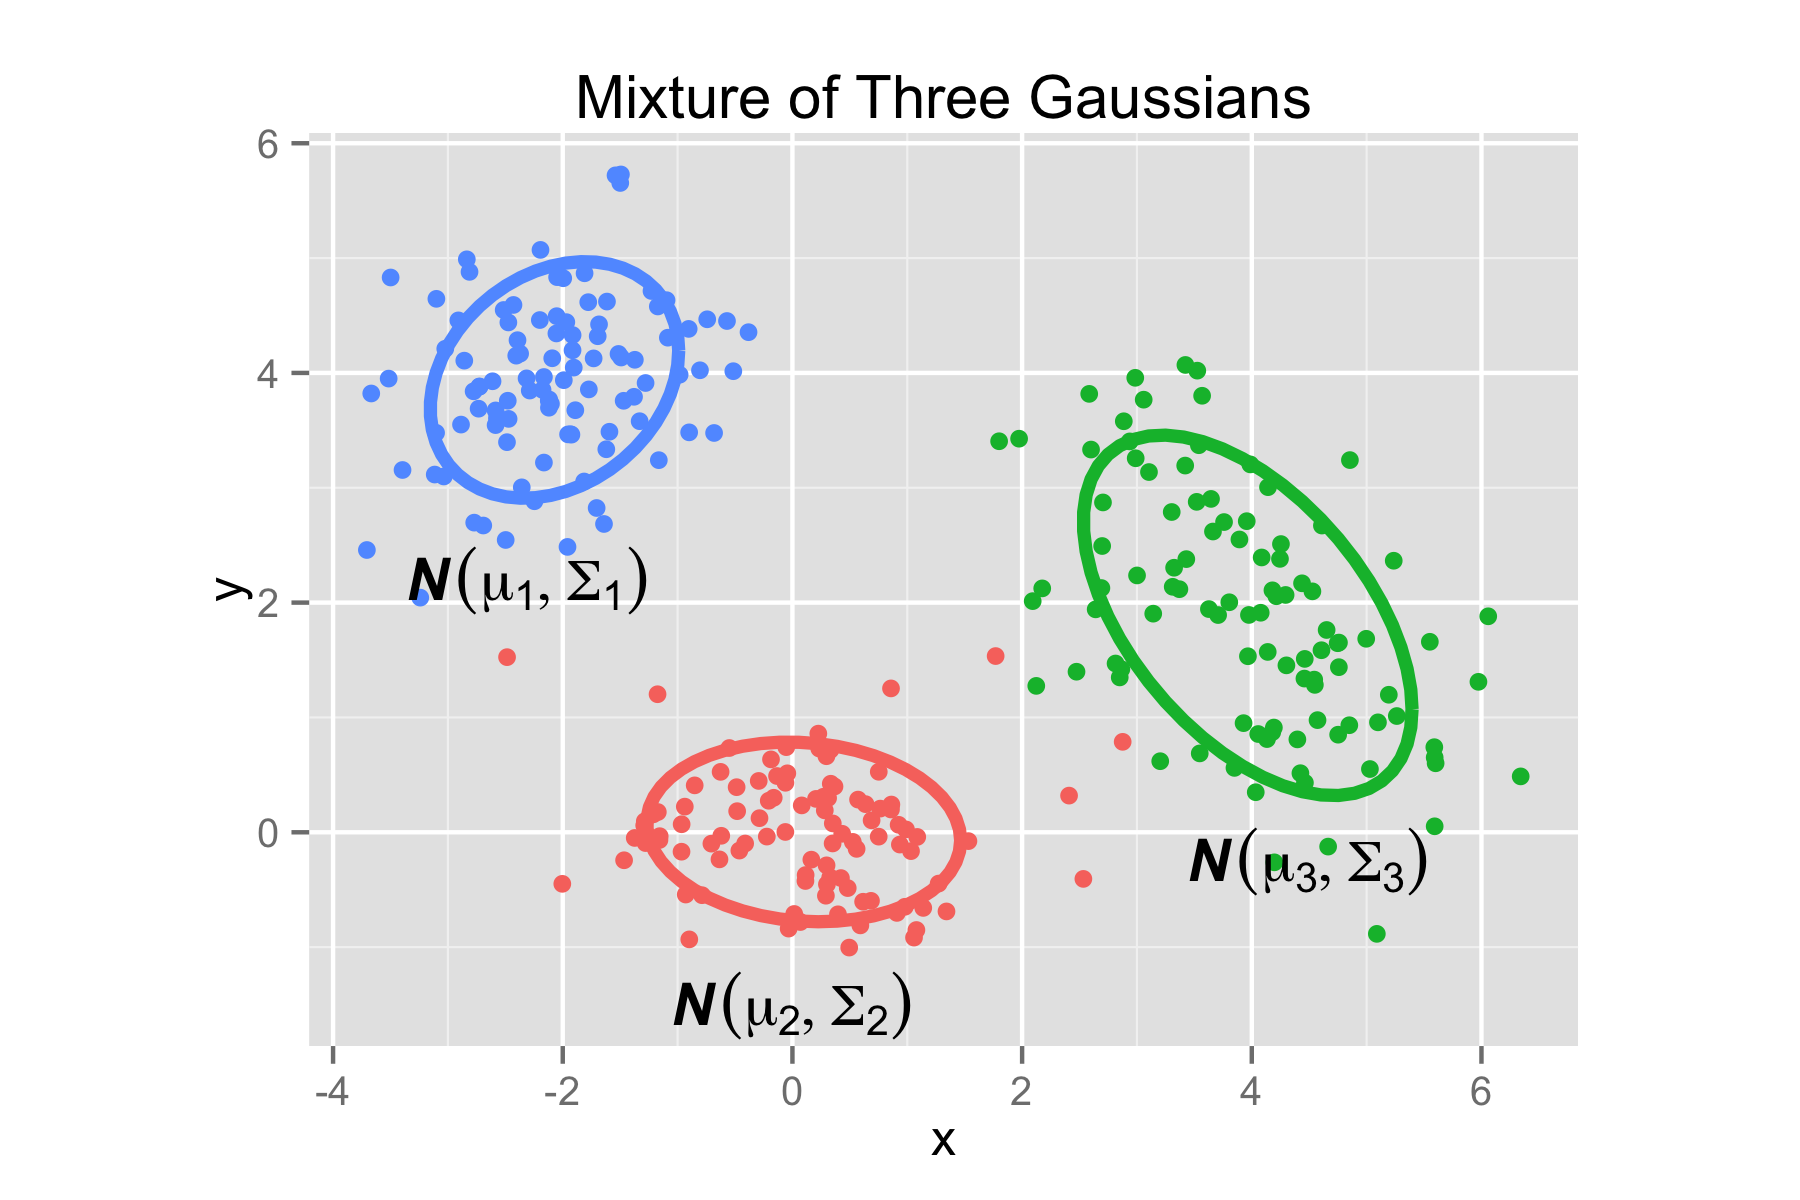
\includegraphics[height=0.5\textheight]{figures/mixture-3-gaussians}

\end{column}
}
\end{columns}
\note[item]{Remember that in probabilistic modeling, we want to model the distribution of $p(y\mid x)$ or $p(x, y)$. Here we don't have $y$, so let's model $p(x)$.}
\end{frame}

\begin{frame}
{Gaussian mixture model (GMM)}
\begin{simpleblock}
{Generative story of GMM with $k$ mixture components:}
\begin{enumerate}
\item Choose cluster $z\sim \text{Categorical}(\pi_1, \ldots, \pi_k)$.
\item Choose $x\mid z \sim \sN(\mu_z, \Sigma_z)$.
\end{enumerate}
\end{simpleblock}

\onslide<2->{
\begin{simpleblock}
{Probability density of $x$:}
\begin{itemize}
\item Sum over (marginalize) the \textbf{latent variable} $z$.
\end{itemize}
\begin{align}
\onslide<.->{p(x) &= \sum_z p(x, z) \\}
        \onslide<.->{&= \sum_z p(x\mid z) p(z) \\}
        \onslide<.->{&= \sum_k \pi_k \sN(\mu_k, \Sigma_k)}
\end{align}
\end{simpleblock}
}
\note[item]{How do we get the prob density of $x$? We know $p(x\mid z)$ and $p(z)$, which means that we know the joint distribution $p(x,z)$.}
\note[item]{Marginalization: expectation of conditional distribution: $\mathbb{E}_{Y}\pb{X\mid Y} = p(X)$.}
\end{frame}

\begin{frame}{Identifiability Issues for GMM}
\begin{itemize}
\item Suppose we have found parameters 
\begin{eqnarray*}
\text{Cluster probabilities}: &  & \pi=\left(\pi_{1},\ldots,\pi_{k}\right)\\
\text{Cluster means}: &  & \mu=\left(\mu_{1},\ldots,\mu_{k}\right)\\
\text{Cluster covariance matrices:} &  & \Sigma=\left(\Sigma_{1},\ldots\Sigma_{k}\right)
\end{eqnarray*}
 that are at a local minimum.
\end{itemize}

\pause{}
\begin{itemize}
\item What happens if we shuffle the clusters? e.g. Switch the labels for
clusters 1 and 2.
\end{itemize}

\pause{}
\begin{itemize}
\item We'll get the same likelihood. How many such equivalent settings are
there?
\end{itemize}

\pause{}
\begin{itemize}
\item Assuming all clusters are distinct, there are $k!$ equivalent solutions.
\end{itemize}

\pause{}
\begin{itemize}
\item Not a problem \emph{per se}, but something to be aware of.
\end{itemize}
\end{frame}
\begin{frame}
{Learning GMMs}
\begin{simpleblock}
{How to learn the parameters $\pi_k, \mu_k, \Sigma_k$?}
\onslide<2->{
\begin{itemize}
\item MLE (also called maximize marginal likelihood).
\item Log likelihood of data:
\begin{align}
L(\theta) &= \sum_{i=1}^n \log p(x_i; \theta) \\
&= \sum_{i=1}^n {\color{red}\log \sum_z} p(x, z; \theta) 
\end{align}
}
\onslide<3->{
\item Cannot push $\log$ into the sum... $z$ and $x$ are coupled.
\item No closed-form solution for GMM---try to compute the gradient yourself!
}
\end{itemize}
\end{simpleblock}
\note[item]{Now that we have $p(x)$, how do we learn the parameters of the distribution?}
\note[item]{The log likelihood is just the log probability of the marginals, so it's also called MML when you have latent variables.}
\note[item]{The log sum term is annoying... That means that $z$ and $x$ are coupled and we probably don't have closed form solution. Recall that previously when we take derivative wrt some parameter $\theta_i$, we can ignore all terms whose subscript is not $i$ and the sums would be simplified.}
\end{frame}

\begin{frame}{Gradient Descent / SGD for GMM}
\begin{itemize}
\item What about running gradient descent or SGD on
\begin{eqnarray*}
J(\pi,\mu,\Sigma) & = & -\sum_{i=1}^{n}\log\left\{ \sum_{z=1}^{k}\pi_{z}\cn\left(x_{i}\mid\mu_{z},\Sigma_{z}\right)\right\} ?
\end{eqnarray*}


\pause{}
\item Can be done, in principle -- but need to be clever about it.

\pause{}
\item Each matrix $\Sigma_{1},\ldots,\Sigma_{k}$ has to be positive semidefinite.

\pause{}
\item How to maintain that constraint?

\pause{}
\begin{itemize}
\item Rewrite $\Sigma_{i}=M_{i}M_{i}^{T}$, where $M_{i}$ is an unconstrained
matrix. 

\pause{}
\item Then $\Sigma_{i}$ is positive semidefinite. 

\pause{}
\end{itemize}
\item Even then, pure gradient-based methods have trouble.\footnote{See Hosseini and Sra's \href{https://arxiv.org/abs/1506.07677}{Manifold Optimization for Gaussian Mixture Models}
for discussion and further references.}
\end{itemize}
\end{frame}


\begin{frame}
{Learning GMMs: observable case}
\begin{simpleblock}
{Suppose we observe cluster assignments $z$. Then MLE is easy:}

\begin{align}
n_{z} &= \sum_{i=1}^{n}\ind{z_{i}=z}
&& \text{\# examples in each cluster}\\
\hat{\pi}(z) &= \frac{n_{z}}{n}
&& \text{fraction of examples in each cluster} \\
\hat{\mu}_{z} &= \frac{1}{n_{z}}\sum_{i:z_{i}=z}x_{i}
&& \text{empirical cluster mean} \\
\hat{\Sigma}_{z} &= \frac{1}{n_{z}}\sum_{i:z_{i}=z}\left(x_{i}-\hat{\mu}_{z}\right)\left(x_{i}-\hat{\mu}_{z}\right)^{T}.
&& \text{empirical cluster covariance}
\end{align}

\end{simpleblock}
\note[item]{Similar to Gaussian NB.}
\note[item]{How do we know $z$?}
\end{frame}

\begin{frame}
{Learning GMMs: inference}
\begin{simpleblock}
{The inference problem: observe $x$, want to know $z$.}
\begin{align}
\onslide<2->{p(z=j \mid x_i) &= p(x, z=j) / p(x) \\}
\onslide<3->{&= \frac{p(x\mid z=j)p(z=j)}{\sum_k p(x\mid z=k) p(z=k)} \\}
\onslide<4->{&= \frac{\pi_j \sN(x_i \mid \mu_j, \Sigma_j)}{\sum_k \pi_k \sN(x_i \mid \mu_k, \Sigma_k)}}
\end{align}
\end{simpleblock}
\onslide<5->{
\begin{itemize}
\item $p(z\mid x)$ is a \emph{soft assignment}.
\item If we know the parameters $\mu, \Sigma, \pi$, this would be easy to compute.
\end{itemize}
}
\note[item]{So now we are in a chicken and egg problem. If we know $z$, the parameters are easy to estimate. If we know the problems, $p(z\mid x)$ is easy to estimate.}
\end{frame}

\begin{frame}
{EM for GMM}
Let's compute the cluster assignments and the parameters iteratively.
\onslide<2->{
\begin{simpleblock}
{The expectation-minimization (EM) algorithm:}
\begin{enumerate}
\item Initialize parameters  $\mu, \Sigma, \pi$ randomly.
\item Run until convergence:
}
\begin{enumerate}
\onslide<3->{
\item E-step: fill in latent variables by inference.
\begin{itemize}
\item compute soft assignments $p(z\mid x_i)$ for all $i$.
\end{itemize}
}
\onslide<4->{
\item M-step: standard MLE for $\mu, \Sigma, \pi$ given ``observed'' variables.
\begin{itemize}
\item Equivalent to MLE in the observable case on data weighted by $p(z\mid x_i)$.
}
\end{itemize}
\end{enumerate}
\end{enumerate}
\end{simpleblock}
\end{frame}

\begin{frame}
{M-step for GMM}
\begin{itemize}
%\item {Recall the gradient is:}
%\begin{align}
%\frac{d }{d \theta} \sum_z \log p(x,z;\theta) = \mathbb{E}_{{\color{red}p(z\mid x)}} \pb{ \frac{d}{d\theta}{\color{blue}\log p(x, z)} } 
%\end{align}
\item Let $p(z\mid x)$ be the soft assignments:
\[
    \gamma_{i}^{j}=\frac{\pi_{j}^{\text{old}}\cn\left(x_{i}\mid\mu_{j}^{\text{old}},\Sigma_{j}^{\text{old}}\right)}{\sum_{c=1}^{k}\pi_{c}^{\text{old}}\cn\left(x_{i}\mid\mu_{c}^{\text{old}},\Sigma_{c}^{\text{old}}\right)} .
\]
\item \think{Exercise}: show that
\begin{eqnarray*}
\mu_{c}^{\text{new}} & = & \frac{1}{n_{c}}\sum_{i=1}^{n}\gamma_{i}^{c}x_{i}\\
\Sigma_{c}^{\text{new}} & = & \frac{1}{n_{c}}\sum_{i=1}^{n}\gamma_{i}^{c}\left(x_{i}-\mu_{c}^{\text{new}}\right)\left(x_{i}-\mu_{c}^{\text{new}}\right)^{T}\\
\pi_{c}^{\text{new}} & = & \frac{n_{c}}{n} .
\end{eqnarray*}
\end{itemize}
\end{frame}

\begin{frame}{EM for GMM}

\begin{itemize}
\item Initialization
\end{itemize}
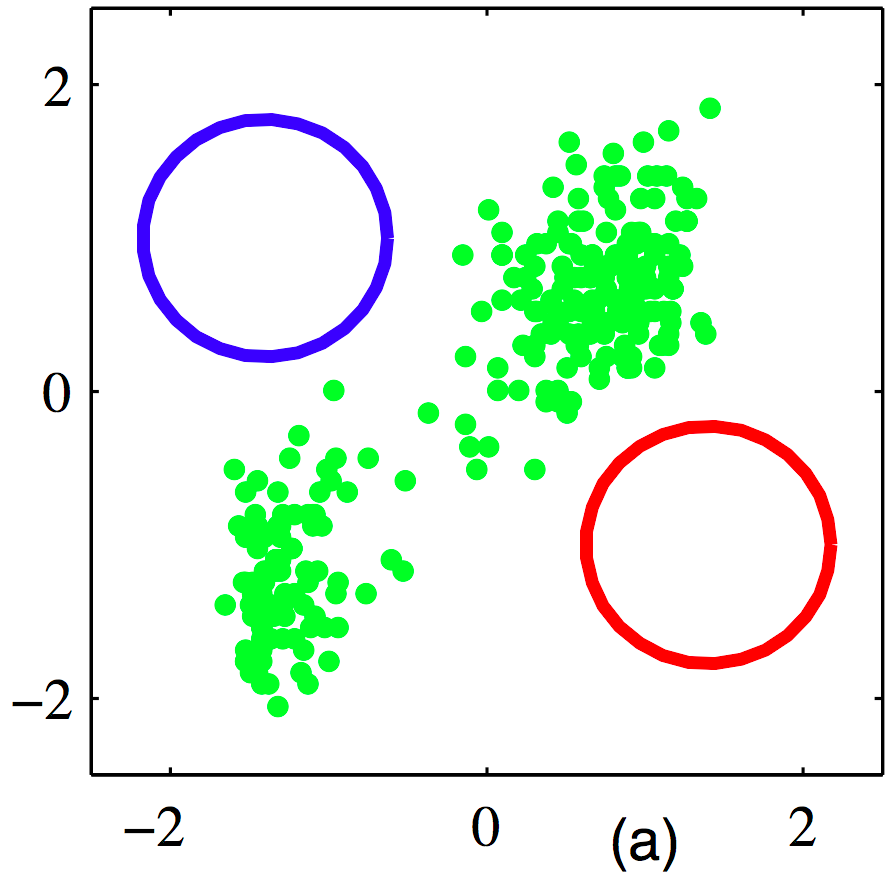
\includegraphics[height=0.55\textheight]{{figures/9.8a}}

\let\thefootnote\relax\footnotetext{\tiny{From Bishop's \emph{Pattern recognition and machine learning}, Figure 9.8.}}
\note[item]{Initially, we have two spherical Gaussian.}
\end{frame}
%
\begin{frame}{EM for GMM}

\begin{itemize}
\item First soft assignment:
\end{itemize}
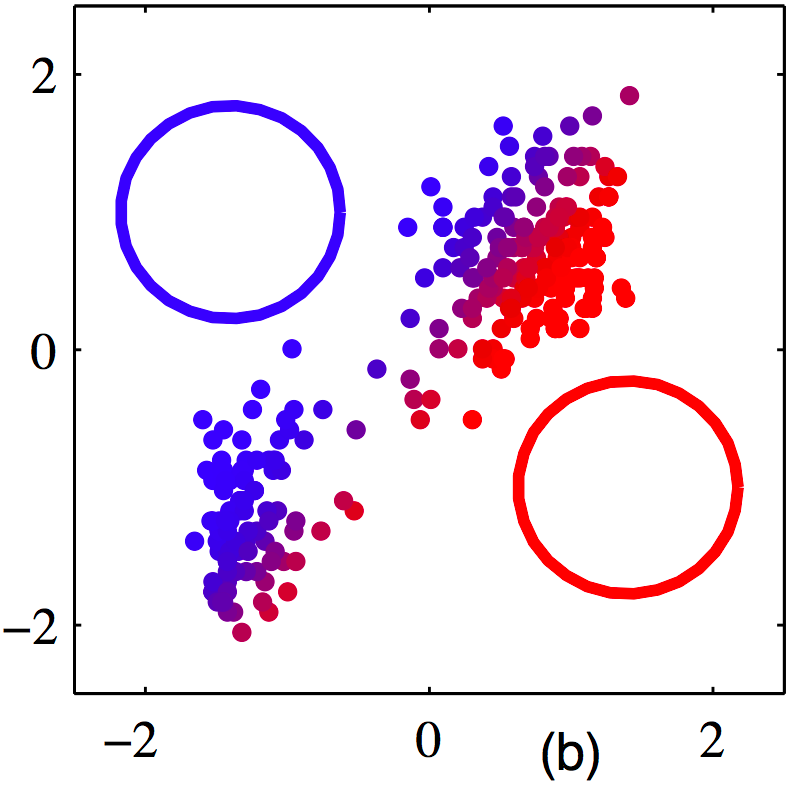
\includegraphics[height=0.55\textheight]{{figures/9.8b}}

\let\thefootnote\relax\footnotetext{\tiny{From Bishop's \emph{Pattern recognition and machine learning}, Figure 9.8.}}
\note[item]{Then we do the soft assignments. The points have mixed cluster membership.}
\end{frame}
%
\begin{frame}{EM for GMM}

\begin{itemize}
\item First soft assignment:
\end{itemize}
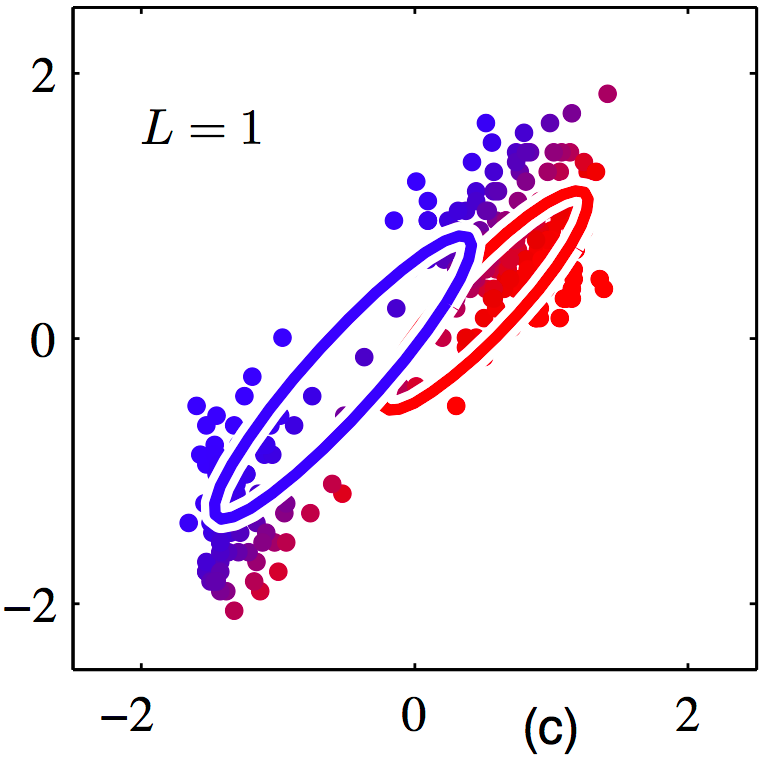
\includegraphics[height=0.55\textheight]{{figures/9.8c}}

\let\thefootnote\relax\footnotetext{\tiny{From Bishop's \emph{Pattern recognition and machine learning}, Figure 9.8.}}
\note[item]{Re-estimate the Gaussians.}
\end{frame}
%
\begin{frame}{EM for GMM}

\begin{itemize}
\item After 5 rounds of EM:
\end{itemize}
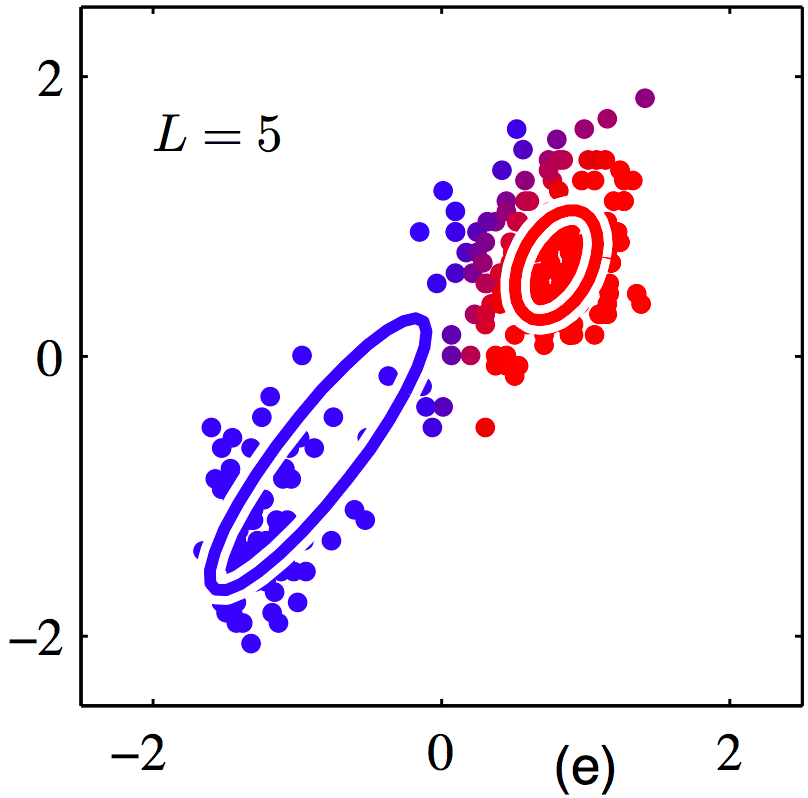
\includegraphics[height=0.55\textheight]{{figures/9.8e}}

\let\thefootnote\relax\footnotetext{\tiny{From Bishop's \emph{Pattern recognition and machine learning}, Figure 9.8.}}

\end{frame}
%
\begin{frame}{EM for GMM}

\begin{itemize}
\item After 20 rounds of EM:
\end{itemize}
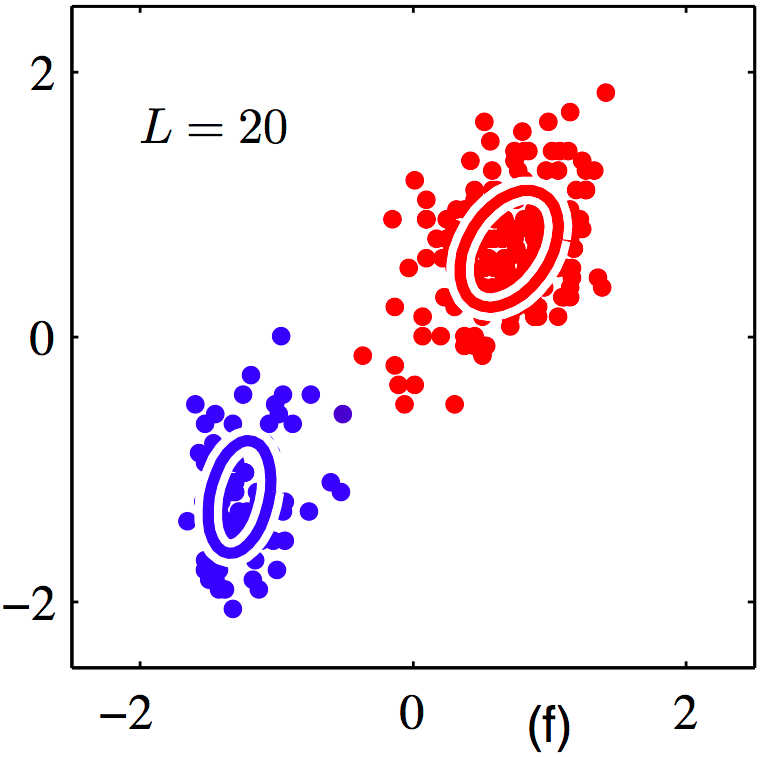
\includegraphics[height=0.55\textheight]{{figures/9.8f}}

\let\thefootnote\relax\footnotetext{\tiny{From Bishop's \emph{Pattern recognition and machine learning}, Figure 9.8.}}
\note[item]{Convergence: likelihood doesn't change much.}
\end{frame}

\begin{frame}
{EM for GMM: Summary}
\begin{itemize}
\item EM is a general algorithm for learning latent variable models.
\item \emph{Key idea}: if data was fully observed, then MLE is easy.
\begin{itemize}
\item E-step: fill in latent variables by computing $p(z\mid x, \theta)$.
\item M-step: standard MLE given fully observed data.
\end{itemize}
\item Simpler and more efficient than gradient methods.
\item Can prove that EM monotonically improves the likelihood and converges to a local minimum.
\item $k$-means is a special case of EM for GMM with \emph{hard assignments}, also called hard-EM.
\end{itemize}
\note[item]{$k$-means: covariance and cluster prior $\pi$ is fixed; only estimate $\mu$; posterior approximated by the delta function.}
\end{frame}

\end{document}
